\chapter{Scheduling}

\epigraph{I wish that I could fly\\
There's danger if I dare to stop and here's the reason why\\
You see I'm overdue\\
I'm in a rabbit stew\\
Can't even say "Good-bye", hello\\
I'm late, I'm late, I'm late\\
No, no, no, no, no, no, no!}{Alice in Wonderland}

CPU Scheduling is the problem of efficiently selecting which process to run on a system's CPU cores.
In a busy system, there will be more ready-to-run processes than there are CPU cores, so the system kernel must evaluate which processes should be scheduled to run and which processes should be executed later.
The system must also decide whetherit should take a particular process and pause its execution -- along with any associated threads.
The balance comes from stopping processes often enough where you have a responsive computer but infrequently enough where the programs themselves are spending minimal time context switching.
It is a hard balance to get right.

The additional complexity of multi-threaded and multiple CPU cores are considered a distraction to this initial exposition so are ignored here.
Another gotcha for non-native speakers is the dual meaning of ``Time'': The word ``Time'' can be used in both clock and elapsed duration context.
For example ``The arrival time of the first process was 9:00am.'' and, ``The running time of the algorithm is 3 seconds''.

One clarification that we will make is that our scheduling will mainly deal with short term or CPU scheduling.
That means we will assume that the processes are in memory and ready to go.
The other types of scheduling are long and medium term.
Long term schedulers act as gatekeepers to the processing world.
When a process requests another process to be executed, it can either tell the process yes, no, or wait.
The medium term scheduler deals with the caveats of moving a process from the paused state in memory to the paused state on disk when there are too many processes or some process are known to use an insignificant amount of CPU cycles.
Think about a process that only checks something once an hour.

\section{High Level Scheduler Overview}

Schedulers are pieces of software programs. In fact, you can implement schedulers yourself!
If you are given a list of commands to exec, a program can schedule them them with SIGSTOP and SIGCONT.
These are called user space schedulers.
Hadoop and python's celery may do some sort of user space scheduling or deal with the operating system.

At the operating system level, you generally have this type of flowchart, described in words first below.
Note, please don't memorize all the states.

\begin{enumerate}
\item New is the initial state. A process has been requested to schedule. All process requests come from fork or clone. At this point the operating system knows it needs to create a new process.
\item A process moves from the new state to the ready. This means any structs in the kernel are allocated. From there, it can go into ready suspended or running.
\item Running is the state that we hope most of our processes are in, meaning they are doing useful work. A process could either get preempted, blocked, or terminate. Preemption brings the process back to the ready state. If a process is blocked, that means it could be waiting on a mutex lock, or it could've called sleep -- either way, it willingly gave up control.
\item On the blocked state the operating system can either turn the process ready or it can go into a deeper state called blocked suspended.
\item There are so-called deep slumber states called blocked suspended and blocked ready. You don't need to worry about these.
\end{enumerate}

We will try to pick a scheme that decides when a process should move to the running state, and when it should be moved back to the ready state.
We won't make much mention of how to factor in voluntarily blocked states and when to switch to deep slumber states.

\section{Measurements}

Scheduling affects the performance of the system, specifically the \emph{latency} and \emph{throughput} of the system.
The throughput might be measured by a system value, for example, the I/O throughput - the number of bits written per second, or the number of small processes that can complete per unit time.
The latency might be measured by the response time -- elapse time before a process can start to send a response -- or wait time or turnaround time --the elapsed time to complete a task.
Different schedulers offer different optimization trade-offs that may be appropriate for desired use.
There is no optimal scheduler for all possible environments and goals.
For example, Shortest Job First will minimize total wait time across all jobs but in interactive (UI) environments it would be preferable to minimize response time at the expense of some throughput, while FCFS seems intuitively fair and easy to implement but suffers from the Convoy Effect.
Arrival time is the time at which a process first arrives at the ready queue, and is ready to start executing.
If a CPU is idle, the arrival time would also be the starting time of execution.

\subsection{What is preemption?}

Without preemption, processes will run until they are unable to utilize the CPU any further.
For example the following conditions would remove a process from the CPU and the CPU would be available to be scheduled for other processes.
The process terminates due to a signal, is blocked waiting for concurrency primitive, or exits normally.
Thus once a process is scheduled it will continue even if another process with a high priority appears on the ready queue.

With preemption, the existing processes may be removed immediately if a more preferred process is added to the ready queue.
For example, suppose at t=0 with a Shortest Job First scheduler there are two processes (P1 P2) with 10 and 20 ms execution times.
P1 is scheduled.
P1 immediately creates a new process P3, with execution time of 5 ms, which is added to the ready queue.
Without preemption, P3 will run 10ms later (after P1 has completed).
With preemption, P1 will be immediately evicted from the CPU and instead placed back in the ready queue, and P3 will be executed instead by the CPU.

Any scheduler that doesn't use some form of preemption can result in starvation because earlier processes may never be scheduled to run (assigned a CPU).
For example with SJF, longer jobs may never be scheduled if the system continues to have many short jobs to schedule.
It all depends on the \href{https://en.wikipedia.org/wiki/Scheduling_(computing)\#Types_of_operating_system_schedulers}{type of scheduler}.

\subsection{Why might a process (or thread) be placed on the ready queue?}

A process is placed on the ready queue when it can use a CPU. Some examples include:

\begin{itemize}
  \tightlist
\item A process was blocked waiting for a \keyword{read} from storage or socket to complete and data is now available.
\item A new process has been created and is ready to start.
\item A process thread was blocked on a synchronization primitive (condition variable, semaphore, mutex lock) but is now able to continue.
\item A process is blocked waiting for a system call to complete but a signal has been delivered and the signal handler needs to run.
\end{itemize}

\section{Measures of Efficiency}

First some definitions

\begin{enumerate}
  \item \keyword{start\_time} is the wall-clock start time of the process (CPU starts working on it)
  \item \keyword{end\_time} is the end wall-clock of the process (CPU finishes the process)
  \item \keyword{run\_time} is the total amount of CPU time required
  \item \keyword{arrival\_time} is the time the process enters the scheduler (CPU may start working on it)
\end{enumerate}

Here are measures of efficiency and their mathematical equations

\begin{enumerate}
\item \keyword{Turnaround Time} is the total time from when the process arrives to when it ends.
  \keyword{end\_time - arrival\_time}
  \item \keyword{Response Time} is the total latency (time) that it takes from when the process arrives to when the CPU actually starts working on it.
    \keyword{start\_time - arrival\_time}
  \item \keyword{Wait Time} is the \emph{total} wait time or the total time that a process is on the ready queue.
    A common mistake is to believe it is only the initial waiting time in the ready queue.
    If a CPU intensive process with no I/O takes 7 minutes of CPU time to complete but required 9 minutes of wall-clock time to complete we can conclude that it was placed on the ready-queue for 2 minutes.
    For those 2 minutes, the process was ready to run but had no CPU assigned.
    It does not matter when the job was waiting, the wait time is 2 minutes.
    \keyword{end\_time - arrival\_time - run\_time}

\end{enumerate}

\subsection{Convoy Effect}

The convoy effect is when a process takes up a lot of the CPU time, leaving all other processes with potentially smaller resource needs following like a Convoy Behind them.

Suppose the CPU is currently assigned to a CPU intensive task and there is a set of I/O intensive processes that are in the ready queue.
These processes require a tiny amount of CPU time but they are unable to proceed because they are waiting for the CPU-intensive task to be removed from the processor.
These processes are starved until the CPU bound process releases the CPU.
But, the CPU will rarely be released.
For example, in the case of an FCFS scheduler, we must wait until the process is blocked due to an I/O request.
The I/O intensive process can now finally satisfy their CPU needs, which they can do quickly because their CPU needs are small and the CPU is assigned back to the CPU-intensive process again.
Thus the I/O performance of the whole system suffers through an indirect effect of starvation of CPU needs of all processes.

This effect is usually discussed in the context of FCFS scheduler; however, a Round Robin scheduler can also exhibit the Convoy Effect for long time-quanta.

\section{Scheduling Algorithms}

Unless otherwise stated

\begin{enumerate}
\item Process 1: Runtime 1000ms
\item Process 2: Runtime 2000ms
\item Process 3: Runtime 3000ms
\item Process 4: Runtime 4000ms
\item Process 5: Runtime 5000ms
\end{enumerate}

\subsection{Shortest Job First (SJF)}

\begin{figure}[H]
\centering
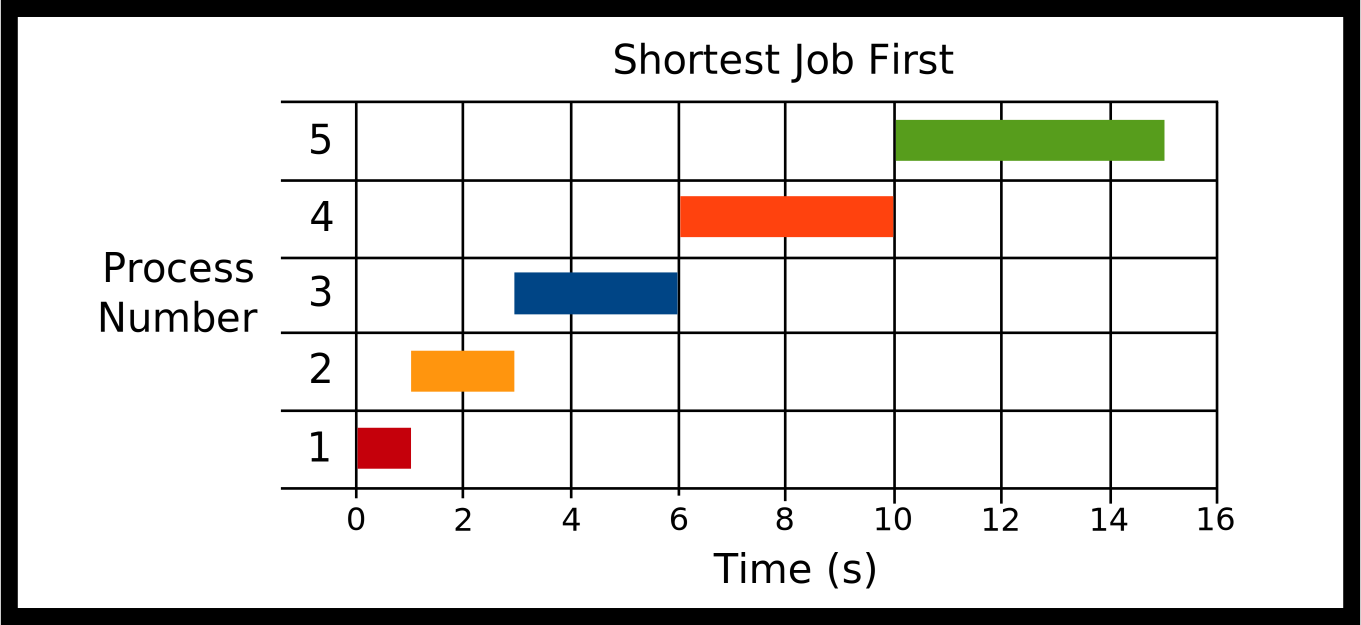
\includegraphics[width=\textwidth]{scheduling/drawings/sjf.eps}
\caption{Shortest job first scheduling}
\end{figure}

\begin{itemize}
\tightlist
\item
  P1 Arrival: 0ms
\item
  P2 Arrival: 0ms
\item
  P3 Arrival: 0ms
\item
  P4 Arrival: 0ms
\item
  P5 Arrival: 0ms
\end{itemize}

The processes all arrive at the start and the scheduler schedules the job with the shortest total CPU time.
The glaring problem is that this scheduler needs to know how long this program will run over time before it ran the program.

Technical Note: A realistic SJF implementation would not use the total execution time of the process but the burst time or the number of CPU cycles needed to finish a program.
The expected burst time can be estimated by using an exponentially decaying weighted rolling average based on the previous burst time \cite[Chapter 6]{silberschatz2005operating}.
For this exposition, we will simplify this discussion to use the total running time of the process as a proxy for the burst time.

\textbf{Advantages}

\begin{enumerate}
  \item Shorter jobs tend to get run first
  \item On average wait times and response times are down
\end{enumerate}

\textbf{Disadvantages}
\begin{enumerate}
  \item Needs algorithm to be omniscient
  \item Need to estimate the burstiness of a process which is harder than let's say a computer network
\end{enumerate}

\subsection{Preemptive Shortest Job First (PSJF)}

Preemptive shortest job first is like shortest job first but if a new job comes in with a shorter runtime than the total runtime of the current job, it is run instead.
If it is equal like our example our algorithm can choose.
The scheduler uses the \emph{total} runtime of the process.
If the scheduler wants to compare the shortest \emph{remaining} time left, that is a variant of PSJF called Shortest Remaining Time First (SRTF).

\begin{figure}[H]
\centering
\includegraphics[width=\textwidth]{scheduling/drawings/psjf.eps}
\caption{Preemptive Shortest Job First scheduling}
\end{figure}

\begin{itemize}
\tightlist
\item
  P2 at 0ms
\item
  P1 at 1000ms
\item
  P5 at 3000ms
\item
  P4 at 4000ms
\item
  P3 at 5000ms
\end{itemize}

Here's what our algorithm does.
It runs P2 because it is the only thing to run.
Then P1 comes in at 1000ms, P2 runs for 2000ms, so our scheduler preemptively stops P2, and let's P1 run all the way through.
This is completely up to the algorithm because the times are equal.
Then, P5 Comes in -- since no processes running, the scheduler will run process 5.
P4 comes in, and since the runtimes are equal P5, the scheduler stops P5 and runs P4.
Finally, P3 comes in, preempts P4, and runs to completion.
Then P4 runs, then P5 runs.

\textbf{Advantages}

\begin{enumerate}
  \item Ensures shorter jobs get run first
\end{enumerate}

\textbf{Disadvantages}

\begin{enumerate}
  \item Need to know the runtime again
  \item Context switching and jobs can get interrupted
\end{enumerate}

\subsection{First Come First Served (FCFS)}

\begin{figure}[H]
\centering
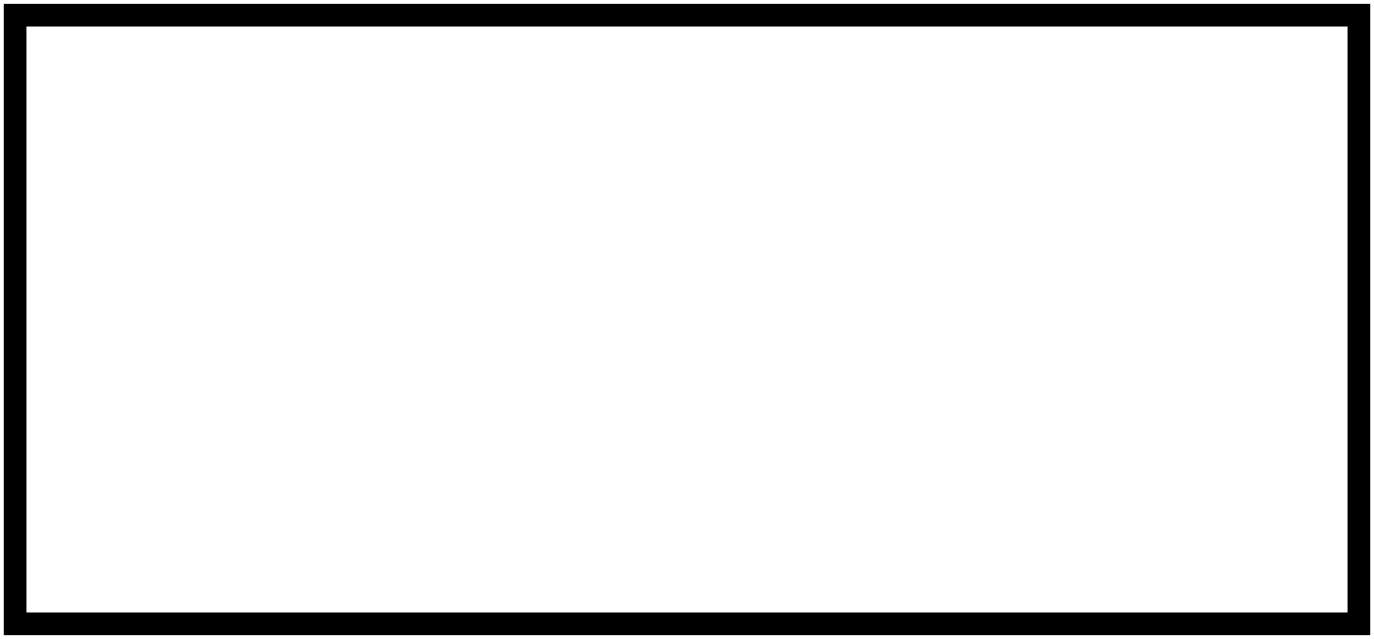
\includegraphics[width=\textwidth]{scheduling/drawings/fcfs.eps}
\caption{First come first serve scheduling}
\end{figure}

\begin{itemize}
\tightlist
\item
  P2 at 0ms
\item
  P1 at 1000ms
\item
  P5 at 3000ms
\item
  P4 at 4000ms
\item
  P3 at 5000ms
\end{itemize}

Processes are scheduled in the order of arrival.
One advantage of FCFS is that scheduling algorithm is simple
The ready queue is a FIFO (first in first out) queue.
FCFS suffers from the Convoy effect.
Here P2 Arrives, then P1 arrives, then P5, then P4, then P3.
You can see the convoy effect for P5.

\textbf{Advantages}

\begin{itemize}
\item Simple algorithm and implementation
\item Context switches infrequent when there are long-running processes
\item No starvation if all processes are guaranteed to terminate
\end{itemize}

\textbf{Disadvantages}
\begin{itemize}
\item Simple algorithm and implementation
\item Context switches infrequent when there are long-running processes

\end{itemize}

\subsection{Round Robin (RR)}

Processes are scheduled in order of their arrival in the ready queue.
After a small time step though, a running process will be forcibly removed from the running state and placed back on the ready queue.
This ensures long-running processes refrain from starving all other processes from running.
The maximum amount of time that a process can execute before being returned to the ready queue is called the time quanta.
As the time quanta approaches to infinity, Round Robin will be equivalent to FCFS.

\begin{figure}[H]
\centering
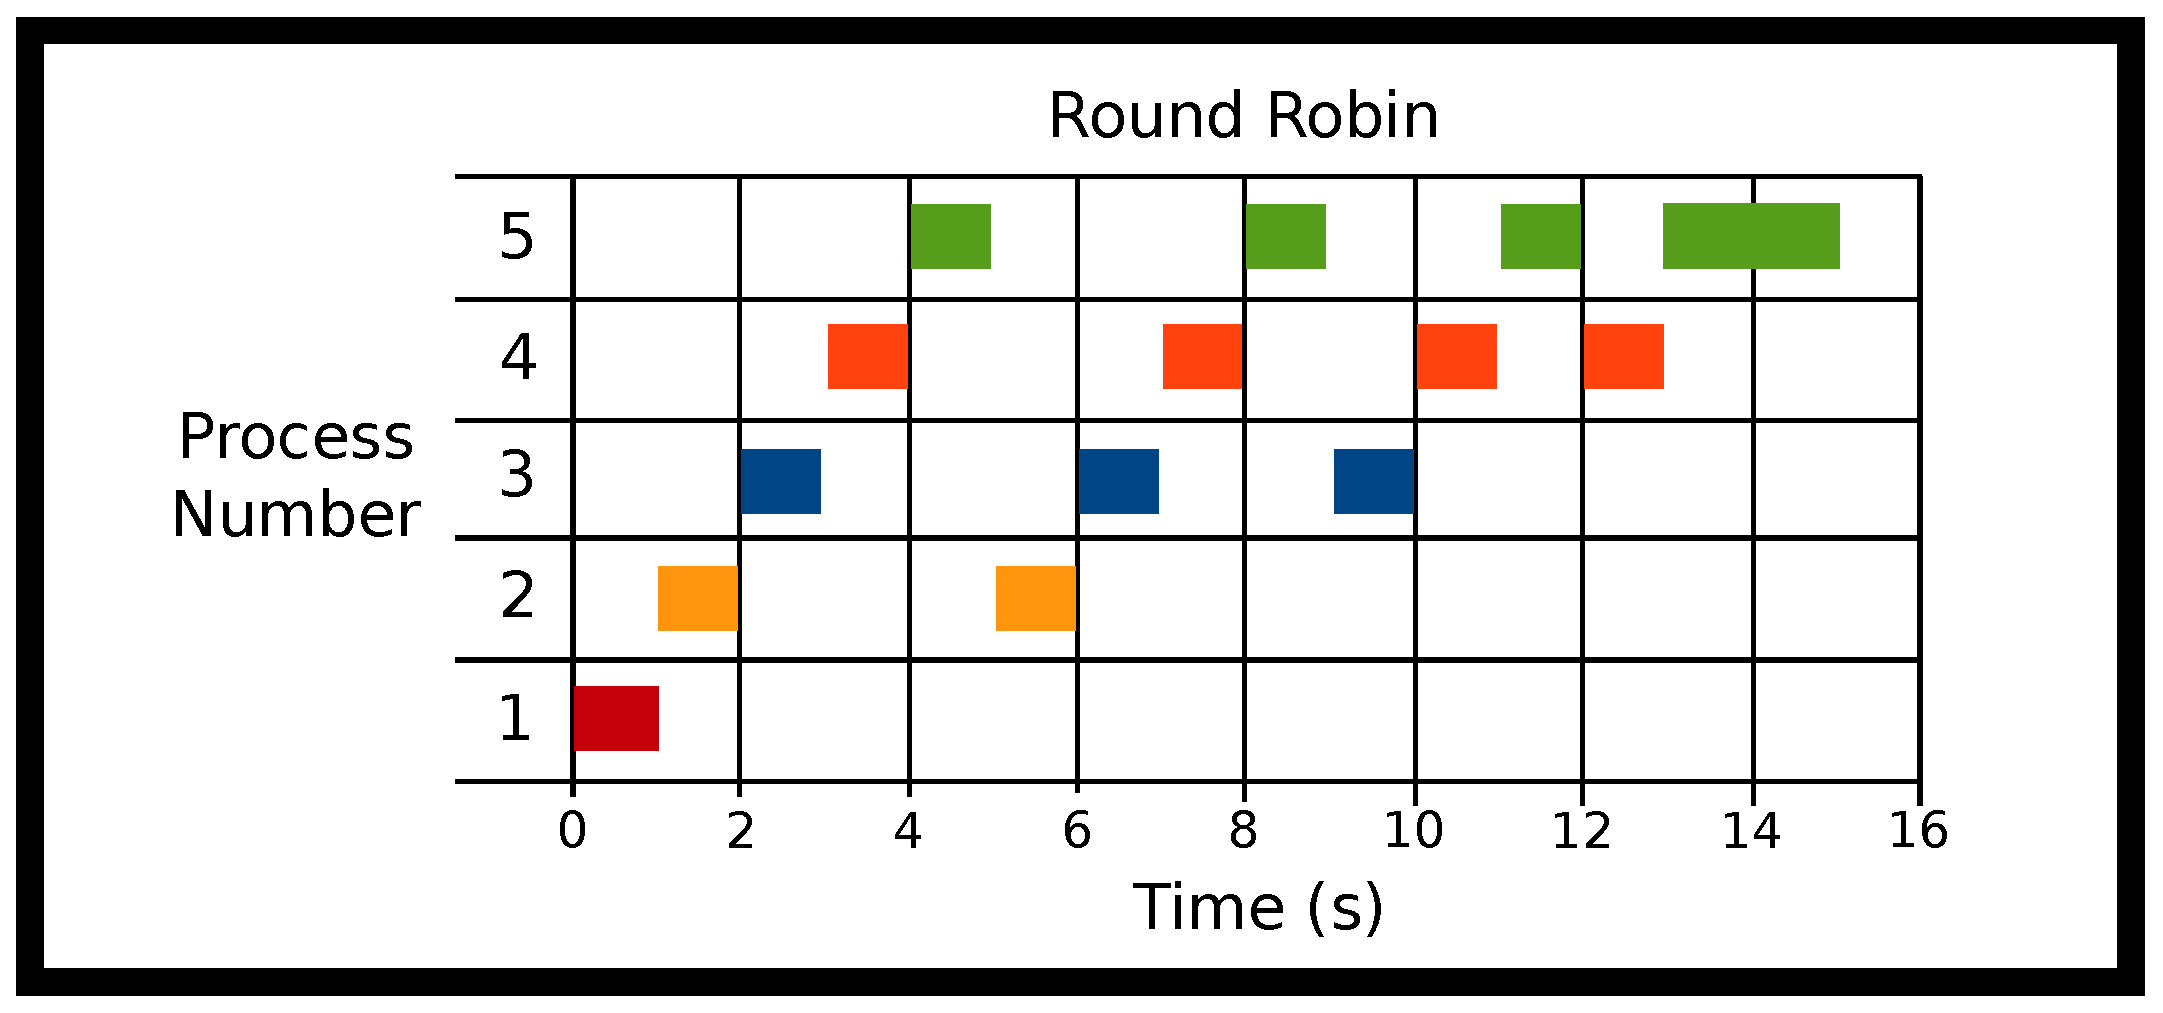
\includegraphics[width=\textwidth]{scheduling/drawings/rr.eps}
\caption{Round Robin Scheduling}
\end{figure}

\begin{itemize}
\tightlist
\item
  P1 Arrival: 0ms
\item
  P2 Arrival: 0ms
\item
  P3 Arrival: 0ms
\item
  P4 Arrival: 0ms
\item
  P5 Arrival: 0ms
\end{itemize}

Quantum = 1000ms

Here all processes arrive at the same time.
P1 is run for 1 quantum and is finished.
P2 for one quantum; then, it is stopped for P3.
After all other processes run for a quantum we cycle back to P2 until all the processes are finished.

\textbf{Advantages}

\begin{enumerate}
  \item Ensures some notion of fairness
\end{enumerate}

\textbf{Disadvantages}

\begin{enumerate}
  \item Large number of processes = Lots of switching
\end{enumerate}

\subsection{Priority}

Processes are scheduled in the order of priority value.
For example, a navigation process might be more important to execute than a logging process.

\textbf{If you need a math-y way of comparing scheduling algorithms, please check out the appendix and the section conceptually scheduling}

\section{Topics}

\begin{itemize}
\tightlist
\item
  Scheduling Algorithms
\item
  Measures of Efficiency
\end{itemize}

\section{Questions}

\begin{itemize}
\tightlist
\item
  What is scheduling?
\item
  What is queueing? What are some different queueing methods?
\item
  What is Turnaround Time? Response Time? Wait Time?
\item
  What is the convoy effect?
\item
  Which algorithms have the best turnaround/response/wait time on average?
\item
  Do preemptive algorithms do better on average response time compared to non preemptive? How about turnaround/wait time?
\end{itemize}

\bibliographystyle{plainnat}
\bibliography{scheduling/scheduling}
